\documentclass[journal]{IEEEtran}
\usepackage{graphicx}
\usepackage{booktabs}
\usepackage{multirow}
\usepackage{float}
\usepackage{placeins}
\usepackage{amsmath}
\usepackage{amssymb}

\graphicspath{{./images/}}

\begin{document}

\title{Supplementary Materials for\\
ADMET-Bench: Task-Dependent Performance of GNNs and Pretrained Models in ADMET Prediction}

\author{}

\maketitle

\renewcommand{\thetable}{S\arabic{table}}
\renewcommand{\thefigure}{S\arabic{figure}}

\section{Architecture-Selection Experiments}
\label{sec:supp_architecture}

This section reports the preliminary architecture-selection screen used to choose the graph neural network backbone. Eight message-passing variants (GraphConv, GCN, GAT, GraphSAGE, GIN, TAG, SGC, and TransformerConv) were evaluated on all six benchmark endpoints under the same scaffold-split pipeline, target transformations, and evaluation metrics used in the main study. For each architecture and endpoint the reported result is the best of five configurations selected on the validation split (search over hidden dimension, number of layers, and learning rate), giving $8 \times 6 \times 5 = 240$ training runs in total.

\begin{table}[H]
\centering
\caption{Preliminary classification architecture screen: test AUC-ROC and F1 on the scaffold-split test set, each architecture at its best of five validation-selected configurations. Best AUC per task in \textbf{bold}.}
\label{tab:arch_classification}
\small
\setlength{\tabcolsep}{4pt}
\begin{tabular}{lcccc}
\toprule
\textbf{Architecture} & \multicolumn{2}{c}{\textbf{Tox21 (NR-AR)}} & \multicolumn{2}{c}{\textbf{hERG}} \\
 & \textbf{AUC} & \textbf{F1} & \textbf{AUC} & \textbf{F1} \\
\midrule
GraphConv & 0.741 & 0.495 & 0.775 & 0.784 \\
GCN & \textbf{0.755} & 0.345 & 0.732 & 0.829 \\
GAT & 0.695 & 0.419 & 0.725 & 0.725 \\
GraphSAGE & 0.711 & 0.329 & 0.785 & 0.863 \\
GIN & 0.724 & 0.481 & 0.733 & 0.841 \\
TAG & 0.726 & 0.247 & 0.765 & 0.813 \\
SGC & 0.708 & 0.409 & \textbf{0.795} & 0.892 \\
Transformer & 0.726 & 0.466 & 0.734 & 0.856 \\
\bottomrule
\end{tabular}
\end{table}

\begin{table}[H]
\centering
\caption{Regression architecture screen: average rank across the four ADME regression datasets (by test R$^2$, lower rank is better), each architecture at its best of five validation-selected configurations. Per-dataset test R$^2$ shown for reference. GraphConv (deployed backbone) in \textbf{bold}.}
\label{tab:arch_regression}
\small
\setlength{\tabcolsep}{4pt}
\begin{tabular}{lccccccc}
\toprule
\textbf{Arch.} & \textbf{Avg Rank} & \textbf{Caco-2} & \textbf{Half-Life} & \textbf{Clear. Hep.} & \textbf{Clear. Mic.} & \textbf{Params} & \textbf{Time (s)} \\
\midrule
GCN & 3.25 & 0.480 & 0.259 & $-$2.039 & 0.227 & 463k & 9.0 \\
Transformer & 3.25 & 0.459 & 0.279 & $-$0.835 & 0.139 & 987k & 12.6 \\
TAG & 4.00 & 0.471 & 0.076 & $-$0.483 & $-$0.494 & 846k & 11.9 \\
\textbf{GraphConv} & 4.75 & 0.443 & $-$0.044 & $-$0.018 & $-$1.911 & 81k & 8.9 \\
SGC & 4.75 & 0.380 & 0.207 & $-$0.144 & $-$0.738 & 180k & 9.4 \\
GAT & 4.75 & 0.368 & 0.288 & $-$1.012 & 0.083 & 145k & 12.8 \\
GIN & 5.00 & 0.487 & $-$0.054 & $-$0.655 & $-$10.000 & 726k & 8.5 \\
GraphSAGE & 6.25 & 0.442 & $-$0.296 & $-$2.660 & 0.133 & 247k & 9.0 \\
\bottomrule
\end{tabular}
\end{table}

No architecture dominates across endpoints: on the structure-driven endpoints the backbones cluster within a narrow band, whereas every architecture collapses to large negative R$^2$ on the weakly-learnable clearance and half-life endpoints. GraphConv was selected because it remains competitive on the learnable endpoints while using only $\approx$81k parameters ($5$--$12\times$ fewer than GCN or TransformerConv) and is among the fastest to train.

\begin{figure}[H]
    \centering
    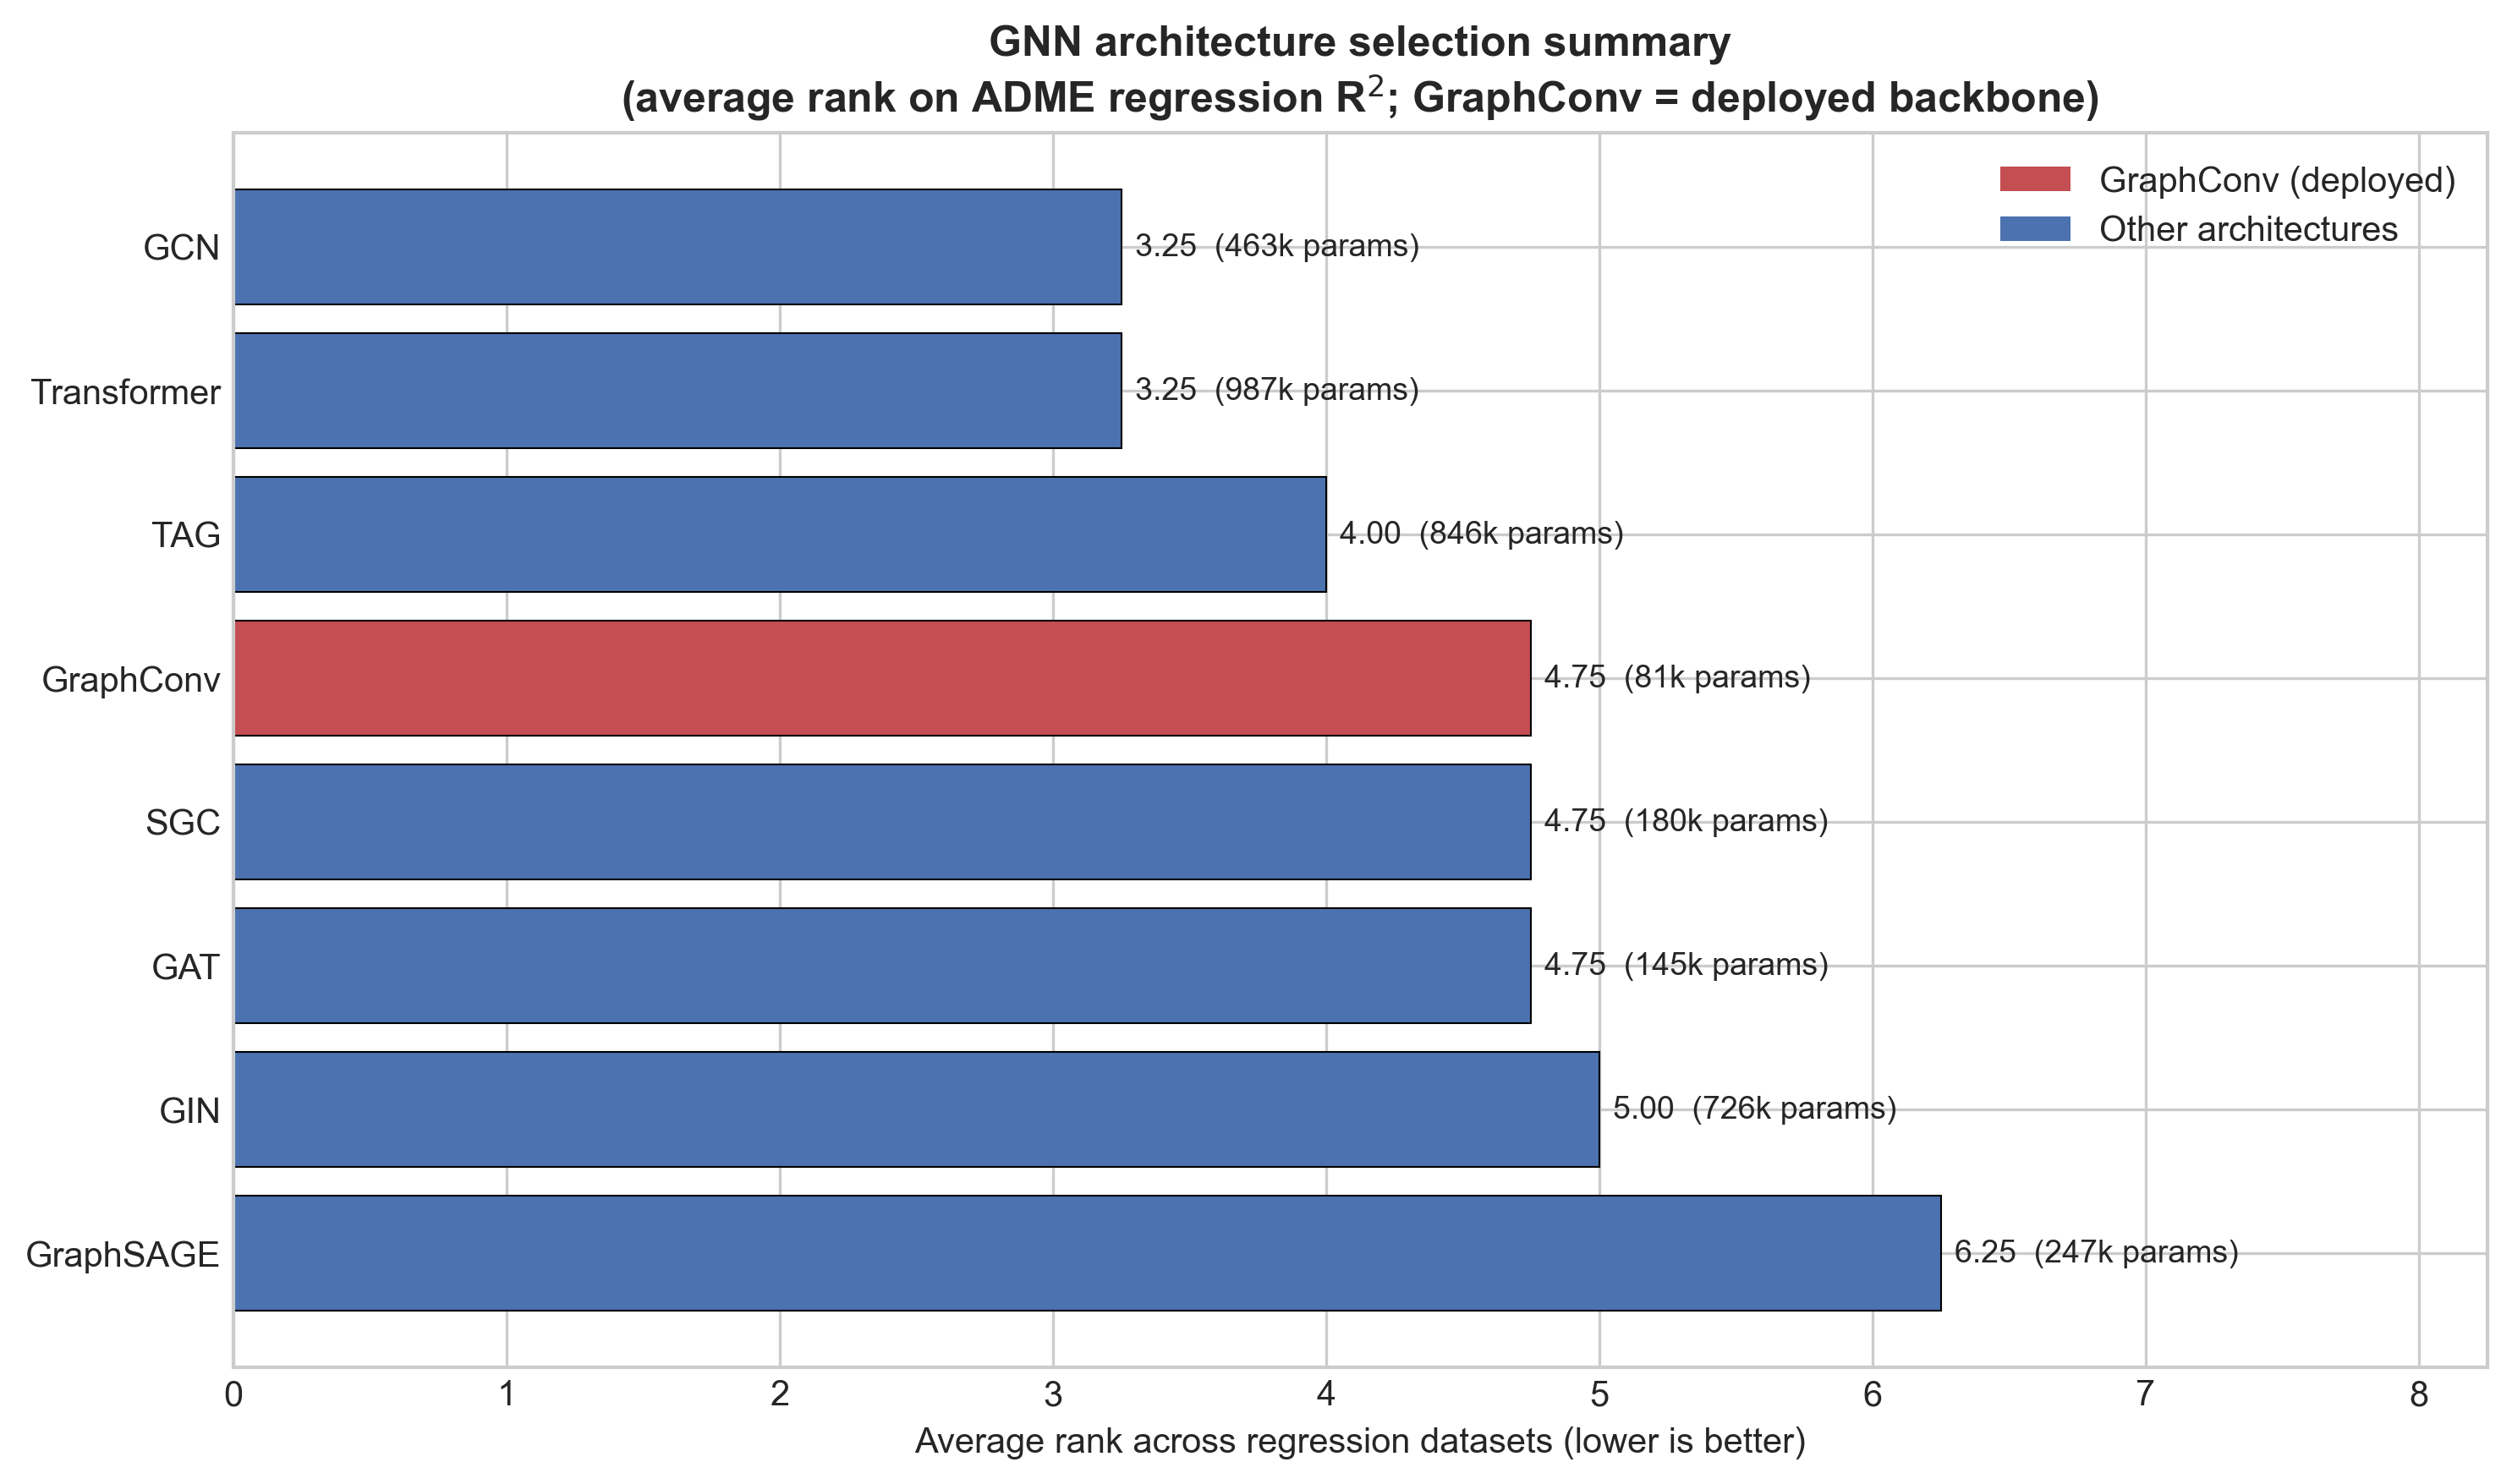
\includegraphics[width=0.95\textwidth,height=0.30\textheight,keepaspectratio]{arch_selection_summary.png}
    \caption{Preliminary architecture-selection summary showing average rank across the regression datasets (lower is better), colored by training stability. GraphConv was selected for its combination of competitive performance, parameter efficiency, and runtime efficiency.}
    \label{fig:arch_selection_summary}
\end{figure}

\begin{figure}[H]
    \centering
    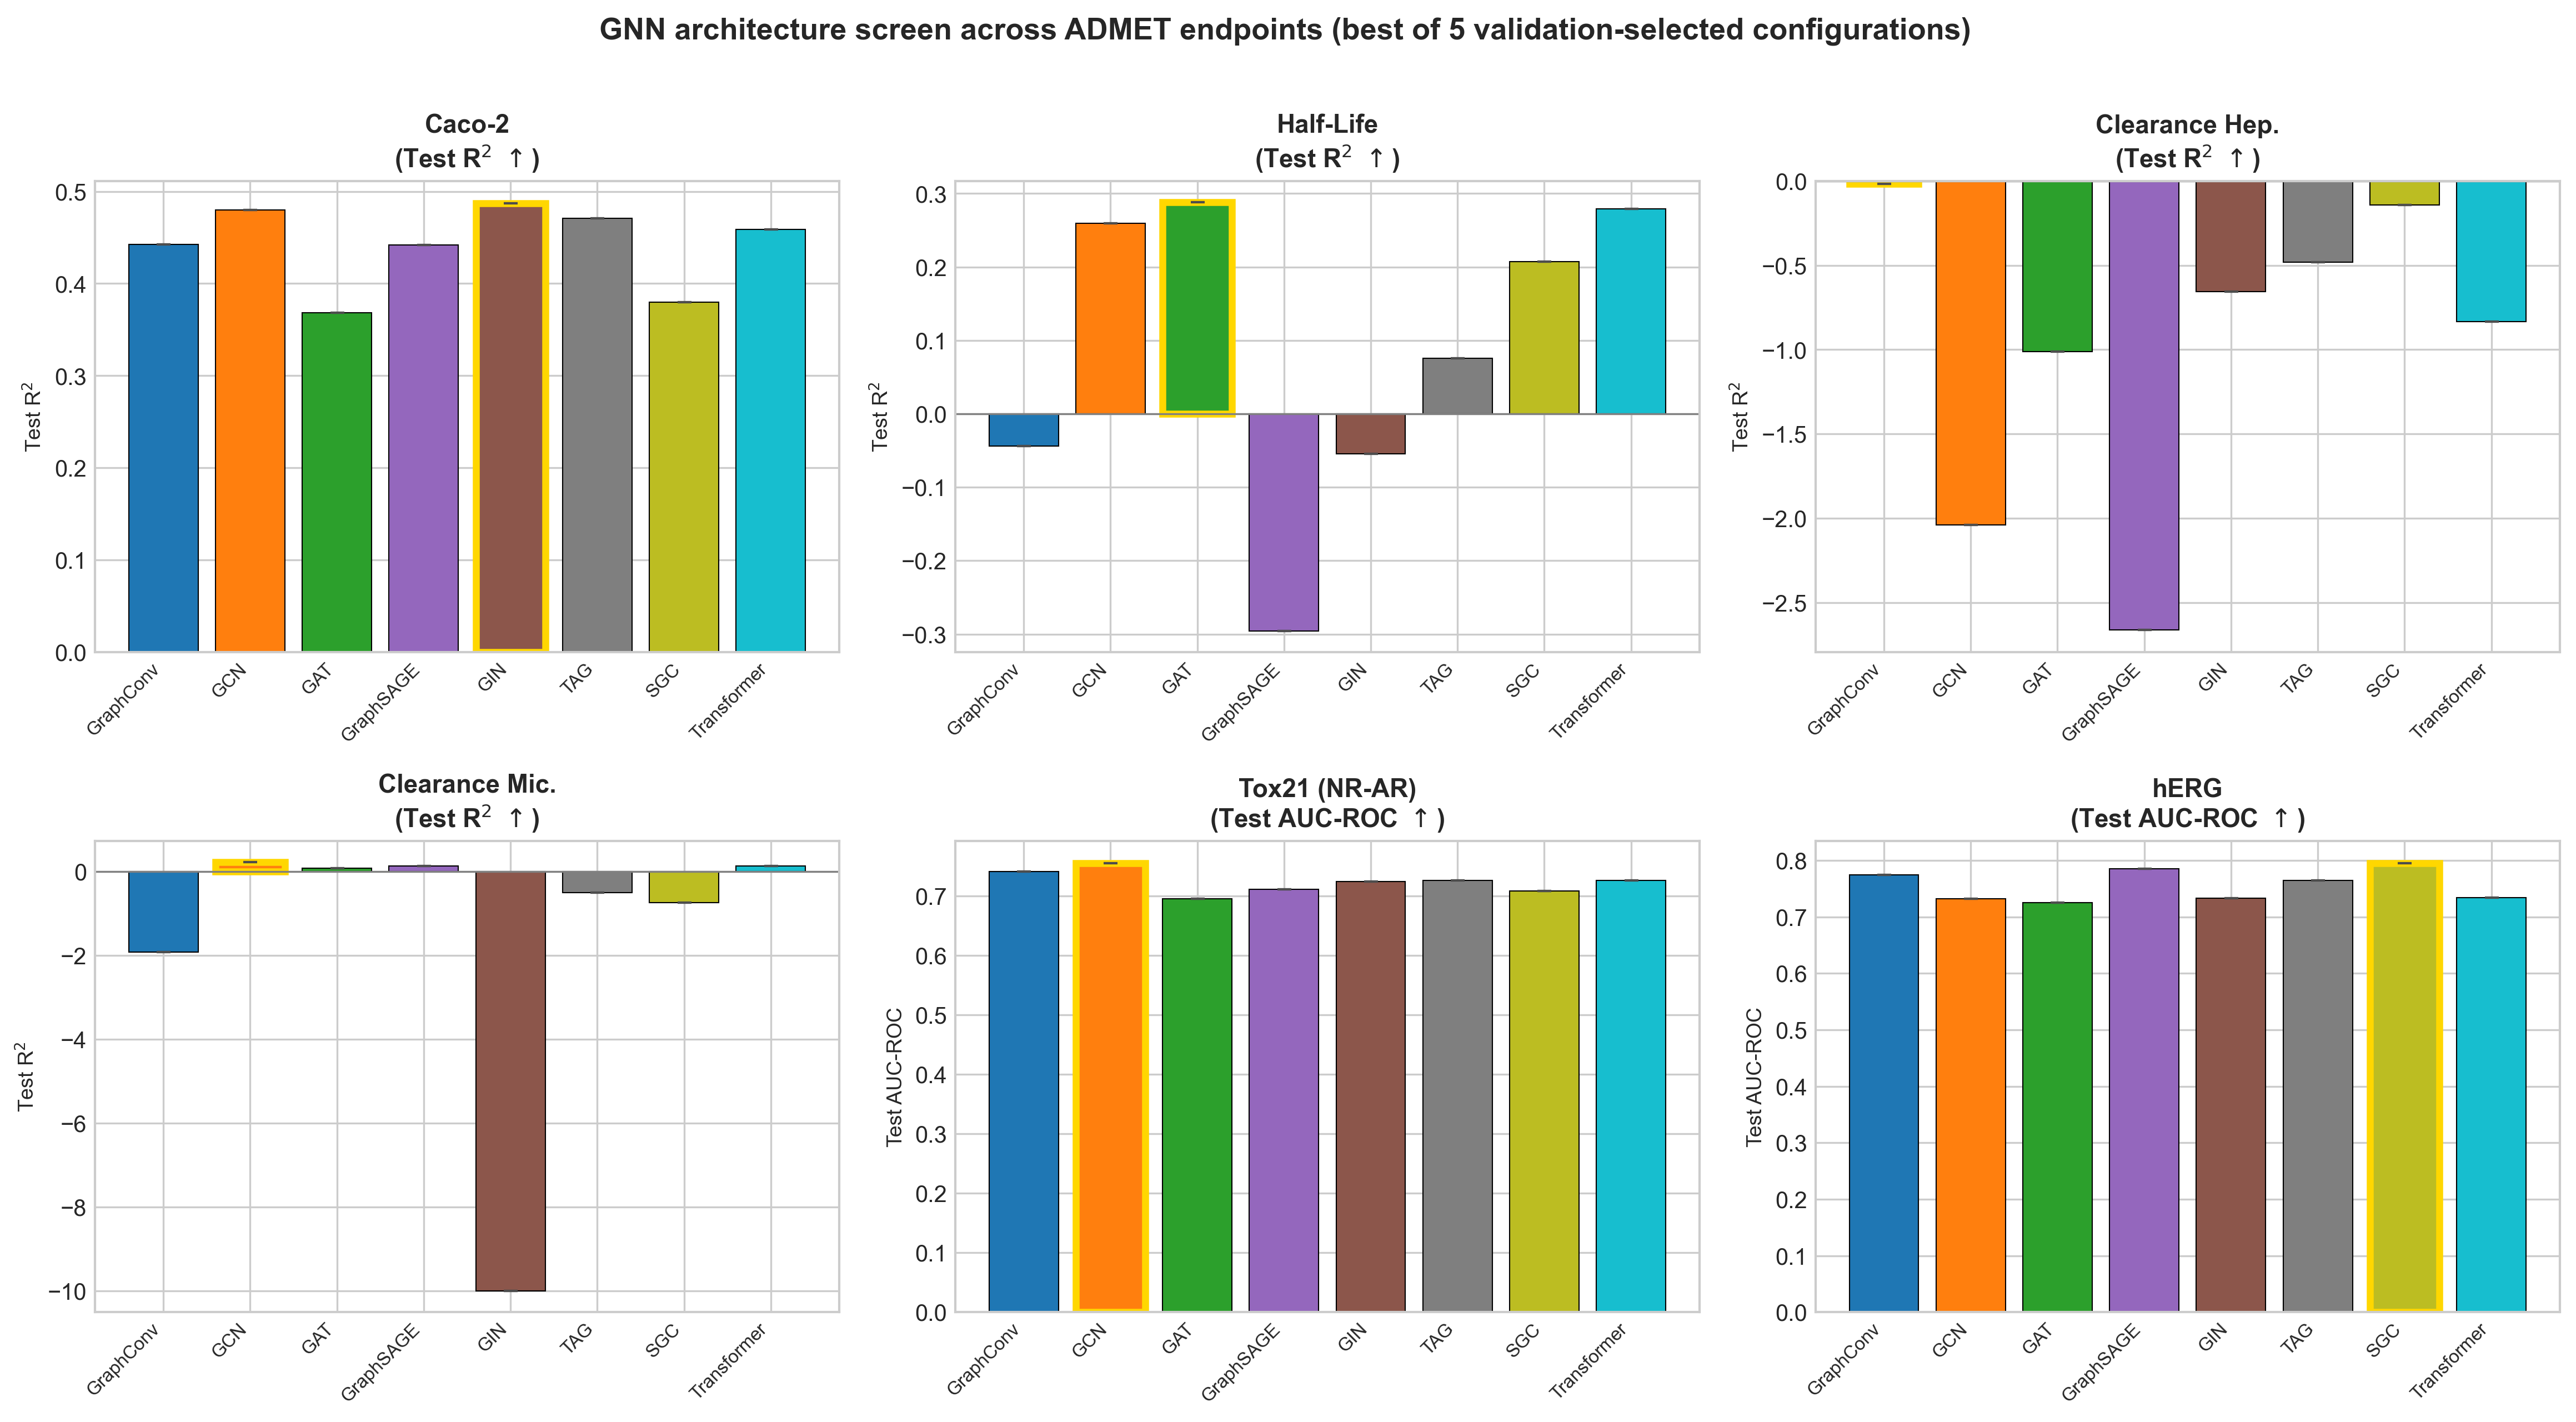
\includegraphics[width=0.95\textwidth,height=0.42\textheight,keepaspectratio]{arch_comparison_all_datasets.png}
    \caption{Per-dataset architecture comparison across all six benchmark endpoints (classification by test AUC-ROC, regression by test R$^2$). The weakly-learnable clearance and half-life endpoints are unstable across all eight architectures, whereas the structure-driven endpoints cluster within a narrow band.}
    \label{fig:arch_comparison}
\end{figure}

\section{Hyperparameter-Optimization Details}
\label{sec:supp_hpo}

\begin{table}[H]
\centering
\caption{HPO algorithms vs.\ Random Search: win/tie/loss, mean relative improvement and bootstrap 95\% confidence intervals across $n$=6 datasets. Improvement direction is normalized so that positive favors the optimizer (RMSE: Random$-$Algo; F1: Algo$-$Random), expressed as a percentage of the Random-Search baseline. CIs are from 10{,}000 percentile bootstrap resamples of the six paired differences; $d_z$ is the paired effect size (mean/std of the differences).}
\label{tab:ci_comparison}
\small
\setlength{\tabcolsep}{4pt}
\begin{tabular}{lcccc}
\toprule
\textbf{Algorithm} & \textbf{W/T/L} & \textbf{Mean $\Delta$ (\%)} & \textbf{95\% CI (\%)} & \textbf{$d_z$} \\
\midrule
PSO & 2/0/4 & $-5.11$ & $[-10.27,\ +0.04]$ & $-0.70$ \\
ABC & 1/0/5 & $-3.92$ & $[-6.96,\ -0.49]$ & $-0.89$ \\
GA  & 2/0/4 & $-4.01$ & $[-9.22,\ +0.92]$ & $-0.57$ \\
SA  & 1/0/5 & $-4.14$ & $[-6.41,\ -1.06]$ & $-1.09$ \\
HC  & 0/0/6 & $-7.04$ & $[-9.54,\ -4.03]$ & $-1.86$ \\
\bottomrule
\end{tabular}
\end{table}

\begin{table}[H]
\centering
\caption{Per-optimizer test F1 on the two classification tasks (single best trial), reported alongside the AUC-ROC of Table~\ref{tab:hpo_results}. These are the F1 values entering the paired comparison against Random Search (Table~\ref{tab:ci_comparison}), with Random Search as the baseline. TPE is omitted because it optimizes a different search space and is excluded from the paired comparison.}
\label{tab:hpo_f1}
\small
\setlength{\tabcolsep}{4pt}
\begin{tabular}{lcccccc}
\toprule
\textbf{Dataset} & \textbf{PSO} & \textbf{ABC} & \textbf{GA} & \textbf{SA} & \textbf{HC} & \textbf{Random} \\
\midrule
Tox21 (NR-AR) & 0.430 & 0.463 & 0.463 & 0.455 & 0.433 & 0.469 \\
hERG & 0.857 & 0.809 & 0.857 & 0.859 & 0.830 & 0.833 \\
\bottomrule
\end{tabular}
\end{table}

\begin{table}[H]
\centering
\caption{Best test set performance per dataset among NiaPy-based HPO algorithms (single best trial). For the regression rows the metric columns report RMSE and R$^2$; for the classification rows they report F1 and AUC-ROC. On Half\_Life\_Obach, PSO, ABC, and GA converged to an identical hyperparameter configuration and are therefore the same trained model, differing only in wall-clock time; the reported ``Best Algo'' reflects the algorithm presentation order used throughout this paper (PSO, ABC, GA, SA, HC, Random), not a performance-based tie-break.}
\label{tab:best_results}
\small
\setlength{\tabcolsep}{4pt}
\begin{tabular}{lcccc}
\toprule
\textbf{Dataset} & \textbf{Best Algo} & \textbf{RMSE/F1} & \textbf{R$^2$/AUC} & \textbf{Time (s)} \\
\midrule
Caco2\_Wang & Random & 0.0027 & 0.481 & 15.7 \\
Half\_Life & PSO & 21.66 & 0.004 & 19.7 \\
Clear.\_Hep. & Random & 68.22 & $-$1.019 & 5.3 \\
Clear.\_Mic. & Random & 38.75 & 0.191 & 52.3 \\
Tox21 (NR-AR) & SA & 0.455 & 0.742 & 1039.6 \\
hERG & ABC & 0.809 & 0.825 & 33.9 \\
\bottomrule
\end{tabular}
\end{table}

\begin{table}[H]
\centering
\caption{Hyperparameter search space for GNN models. The three MLP-head layer widths are sampled independently and then sorted in descending order (Layer~1~$\geq$~Layer~2~$\geq$~Layer~3) to yield a funnel-shaped prediction head.}
\label{tab:search_space}
\small
\begin{tabular}{ll}
\toprule
\textbf{Hyperparameter} & \textbf{Search Space} \\
\midrule
Hidden Dimensions & \{64, 96, 128, 192, 256, 384, 512\} \\
Number of Layers & \{3, 4, 5, 6, 7\} \\
Learning Rate & [1e-4, 1e-2] (log-uniform) \\
Weight Decay & [1e-6, 1e-2] (log-uniform) \\
MLP Head Layer 1 & \{128, 192, 256, 384, 512\} \\
MLP Head Layer 2 & \{64, 96, 128, 192, 256\} \\
MLP Head Layer 3 & \{32, 48, 64, 96, 128\} \\
\bottomrule
\end{tabular}
\end{table}

\begin{table*}[!t]
\centering
\caption{HPO algorithm comparison across datasets. Values show test metrics for each optimizer. Best per dataset in \textbf{bold}. TPE operates over a slightly expanded search space that includes dropout.}
\label{tab:hpo_results}
\scriptsize
\begin{tabular}{lccccccc}
\toprule
\textbf{Dataset} & \textbf{PSO} & \textbf{ABC} & \textbf{GA} & \textbf{SA} & \textbf{HC} & \textbf{Random} & \textbf{TPE} \\
\midrule
\multicolumn{8}{l}{\emph{Regression (RMSE $\downarrow$)}} \\
\midrule
Caco2\_Wang & 0.0031 & 0.0029 & 0.0031 & 0.0029 & 0.0030 & \textbf{0.0027} & 0.0029 \\
Half\_Life\_Obach & 21.66 & 21.66 & 21.66 & 23.70 & 24.52 & 22.31 & \textbf{21.48} \\
Clearance\_Hep. & 70.21 & 72.04 & 71.34 & 72.04 & 72.04 & \textbf{68.22} & 80.32 \\
Clearance\_Mic. & 42.76 & 42.29 & 42.29 & 40.94 & 41.63 & \textbf{38.75} & 40.89 \\
\midrule
\multicolumn{8}{l}{\emph{Classification (AUC-ROC $\uparrow$)}} \\
\midrule
Tox21 (NR-AR) & 0.692 & 0.735 & 0.735 & \textbf{0.742} & 0.652 & 0.713 & 0.722 \\
hERG & 0.747 & \textbf{0.825} & 0.747 & 0.802 & 0.821 & 0.747 & 0.756 \\
\bottomrule
\end{tabular}
\end{table*}

\begin{figure}[!t]
    \centering
    
\includegraphics[width=\columnwidth,height=0.28\textheight,keepaspectratio]{confusion_matrices.png}
    \caption{Confusion matrices for the best-performing toxicity classification models. (A) Tox21 shows majority-class bias due to extreme imbalance (SA, F1 = 0.455). (B) hERG shows balanced performance (ABC, F1 = 0.809).}
    \label{fig:confusion_matrices}
\end{figure}

\begin{figure}[!t]
    \centering
    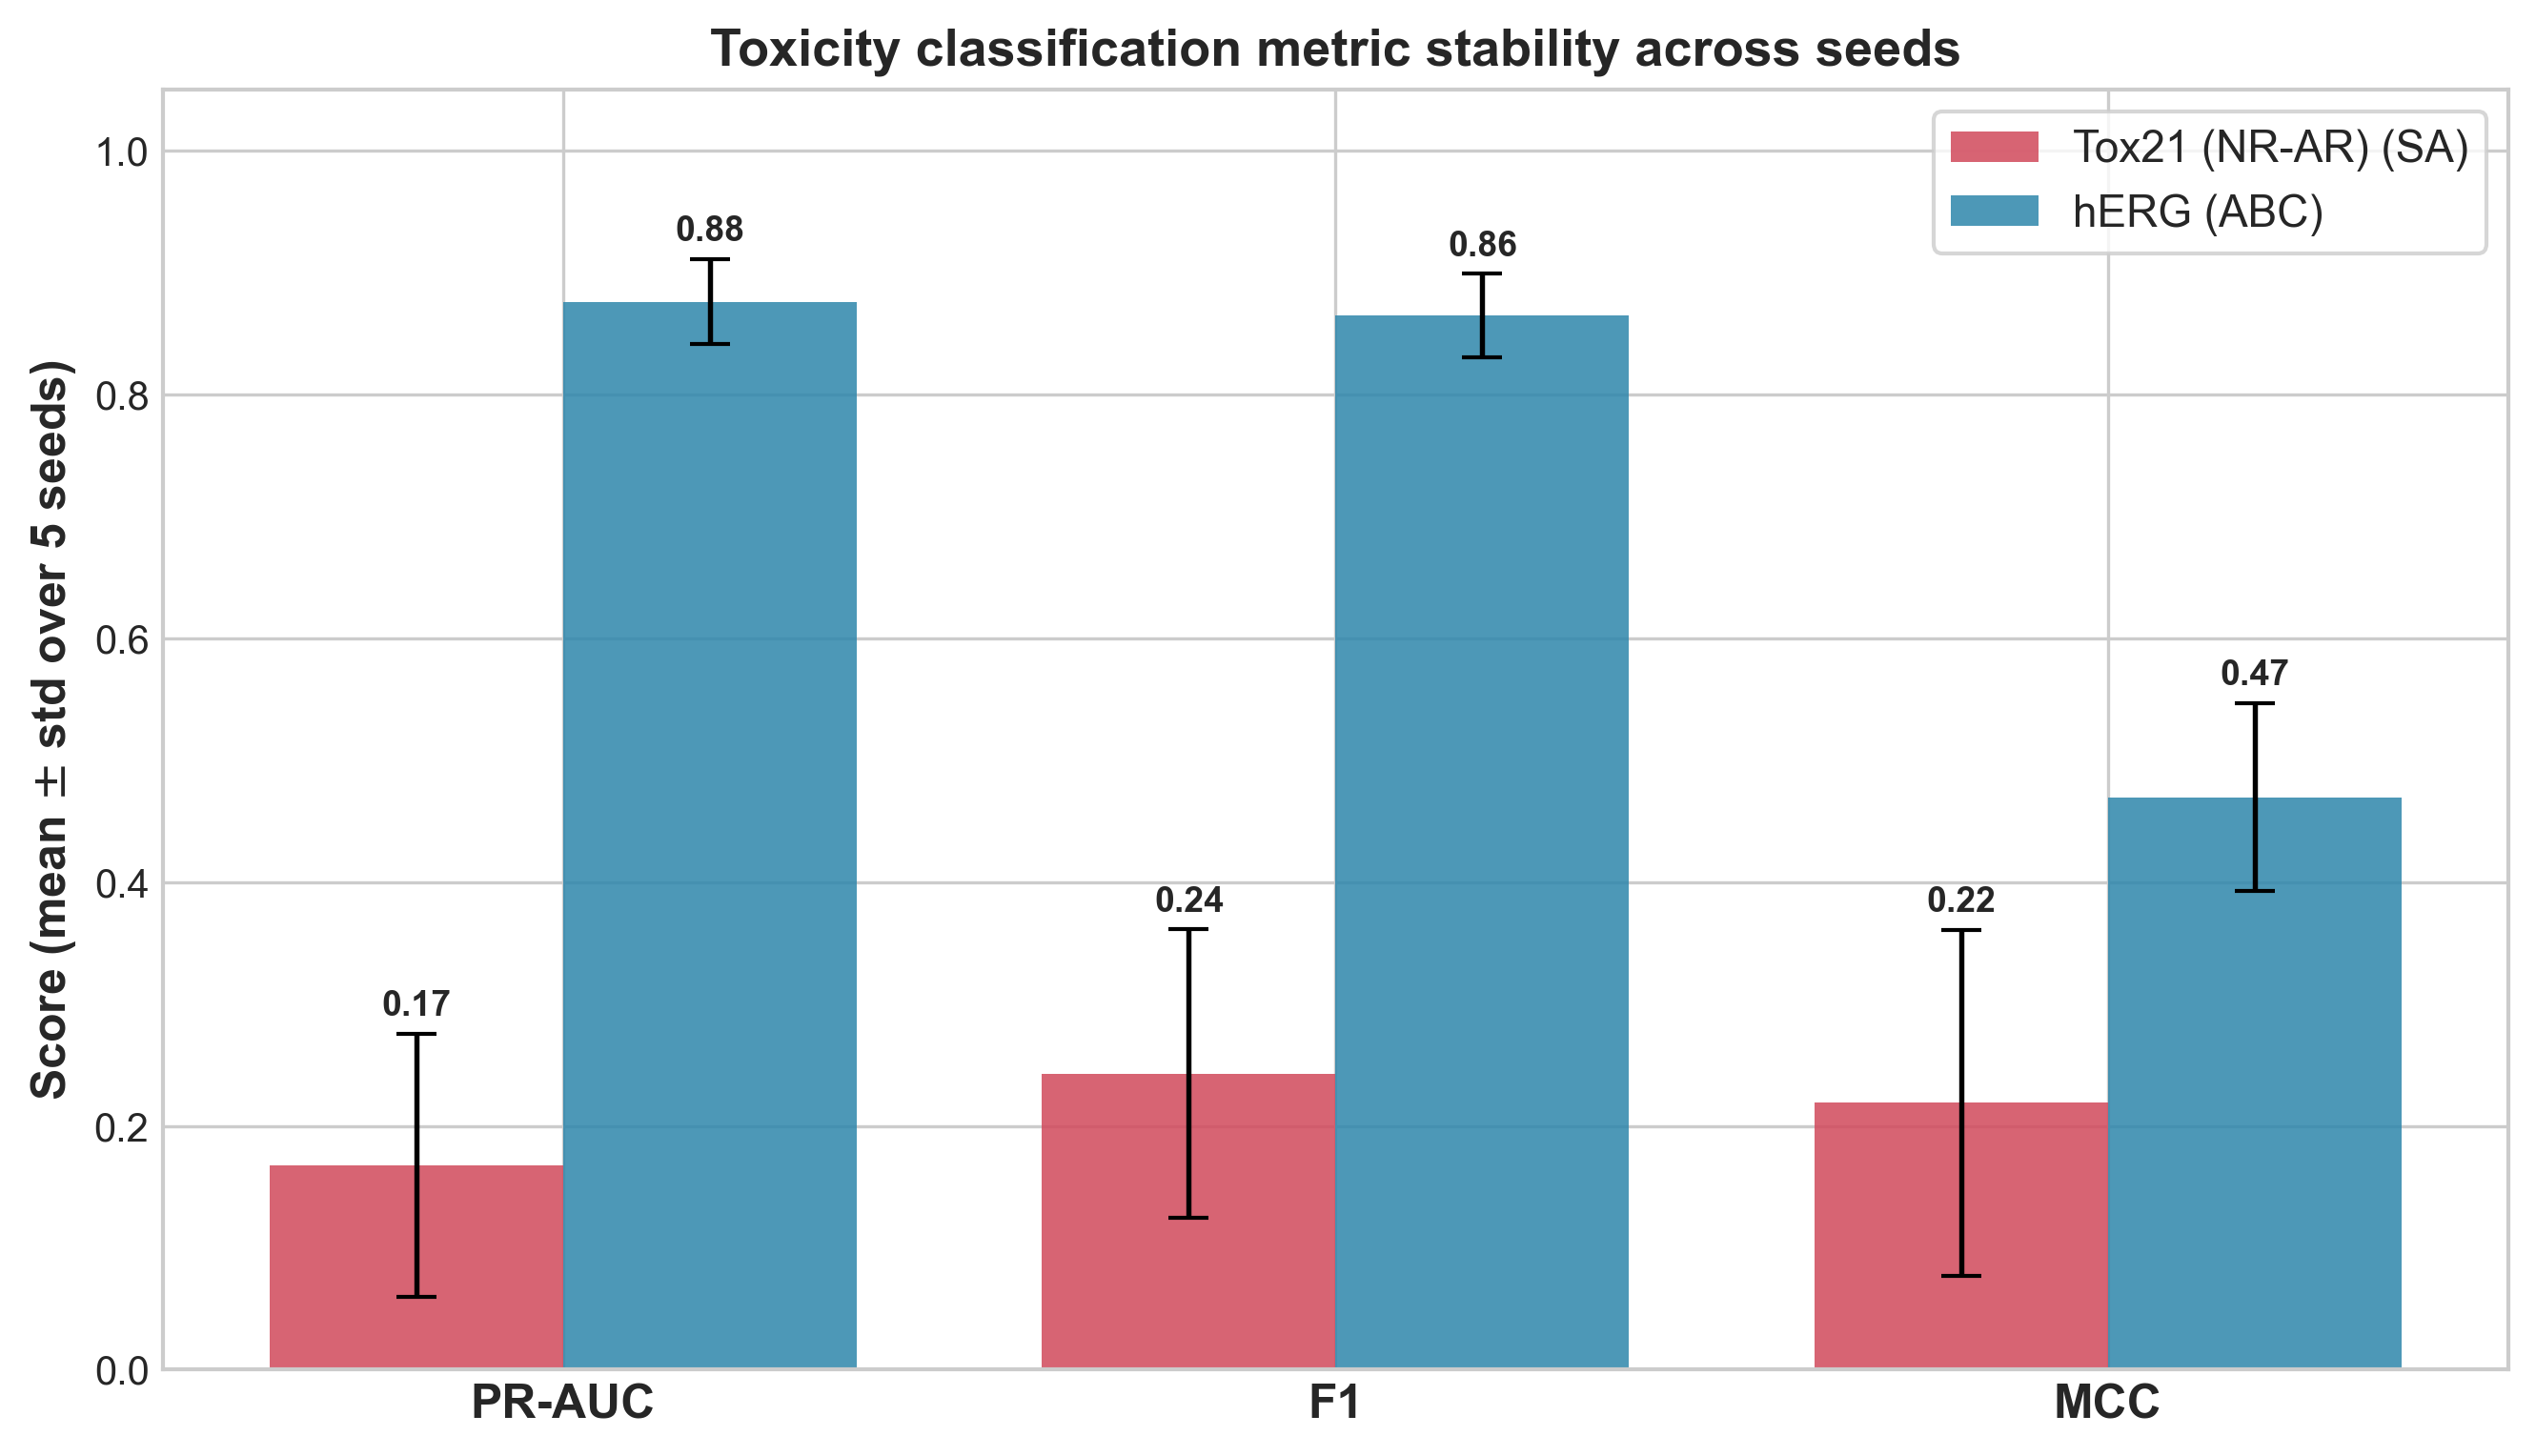
\includegraphics[width=\columnwidth,height=0.30\textheight,keepaspectratio]{toxicity_metric_stability.png}
    \caption{Across-seed stability of the imbalance-aware toxicity metrics (PR-AUC, F1, MCC). Bars show the mean over five seeds and error bars show $\pm$ one standard deviation. These imbalance-aware summaries use mean $\pm$ standard deviation to quantify across-seed variability; the primary AUC-ROC results are summarized using median [min--max] in the main manuscript. Variability is small for hERG but large for Tox21, reflecting the instability induced by extreme class imbalance.}
    \label{fig:toxicity_stability}
\end{figure}

\begin{figure*}[!t]
    \centering
    
\includegraphics[width=\textwidth,height=0.42\textheight,keepaspectratio]{hpo_convergence_curves.png}
    \caption{Convergence trajectories for HPO algorithms across all six benchmark datasets (four ADME regression and two toxicity classification tasks), showing the best-so-far validation metric per training epoch for the best configuration selected by each algorithm. The curves illustrate qualitative optimization behavior recorded during the HPO analysis.}
    \label{fig:convergence}
\end{figure*}

\end{document}
